\documentclass{article}
\usepackage[utf8]{inputenc}
\usepackage{listings}
\usepackage{float}
\usepackage{graphicx}
\graphicspath{{images/}{../images/}}


\title{Databases Summary 2018}
\author{Jacob Burley}
\date{Block 5 2018}

\begin{document}
%TODO: organisation
%       questionable/unquestionable functional dependency
\long\def\/*#1*/{}
\restylefloat{table}
\maketitle

\section*{Lecture 1}
\subsection*{Transactions}
A transaction is a collection of operations that performs a single \textbf{logical} function within a database application.
\\The \textbf{Transaction Management Component} ensures that the database remains in a consistent (aka correct) state, even if a \textbf{system failure} (e.g. power loss, OS crash etc) or a \textbf{transaction failure} occurs.
\\We also have a \textbf{Concurrency Control Manager} that controls the interactions between any concurrent transactions, helping to make sure that the database remains in a consistent state.

\subsection*{ACID properties}
These properties of a Database Management System are critical in order to maintain the consistency of the database, as mentioned above.
\begin{itemize}
    \item \textbf{Atomicity:} The transaction either is completed (it commits), or it doesn't impact the database at all (it aborts)
    \item \textbf{Consistency:} The transaction always leaves the database in a consistent state. This means that all defined \textbf{integrity constraints} hold.
    \item \textbf{Isolation:} Multiple users can modify the same database concurrently, but their transactions will not be visible to other users while incomplete. Essentially, the final system state is the same as what would be obtained if all the transactions would be executed in sequence.
    \item \textbf{Durability:} Once a transaction has committed successfully, the modified data persists, even if there is a system failure such as a disk crash.
\end{itemize}
\newpage    
\section*{Lecture 2}
\subsection*{Relational Model}
Also known as "rectangular tables"
\begin{itemize}
    \item The \textbf{Schema} is the structure of the database, which is the same as the \textbf{relations + constraints}.
    \item A \textbf{database} is a set of named \textbf{relations} (\textbf{tables})
    \item Each relation in a database has a set of named \textbf{attributes} (\textbf{columns})
    \item Each \textbf{tuple} (\textbf{row}) has a value for each attribute
    \begin{itemize}
        \item A tuple may contain NULL values, indicating that a value is unknown or undefined.
        \item NULL values can be disallowed by the datatype of the attribute, which would mean that attempting to insert a tuple containing a null value would result in failure. For example, if we wanted a \verb|VARCHAR| field to not allow null, we would declare it as \verb|VARCHAR(20) NOT NULL| in SQL.
        \item NULL values being disallowed can lead to users inventing fake values to fill missing columns. This is bad as it can, for example, affect data analysis done on this data in the future.
        \item NULL is \textbf{not} the same as the number 0, and is also \textbf{not} the same as an empty string. It is its own datatype.
        \item There is no clear definition of how to use null. SQL uses \textbf{three-valued logic} (true, false, unknown) for the evaluation of comparisons involving null values.
    \end{itemize}
    \item Each attribute has a \textbf{datatype} (\textbf{domain})
    \item A \textbf{key} is an attribute whose value is unique in each tuple.
    \begin{itemize}
        \item A key can also be a set of attributes whose combined values are unique
        \item We can indicate a key in a schema by \underline{underlining} the attribute(s) that make(s) up the key
    \end{itemize}
\end{itemize}
\subsubsection*{Creating a table using a relation schema}
\begin{table}[H]
\begin{center}
 \begin{tabular}{| c | c | c | c |} 
 \hline
 \underline{\texttt{CAT}} & \underline{\texttt{ENO}} & \texttt{TOPIC} & \texttt{MAXPT} \\ [0.5ex] 
 \hline
 H & 1 & Rel.Alg. & 10 \\
 H & 2 & SQL & 10 \\
 H & 1 & SQL & 14 \\
 \hline
\end{tabular}
\end{center}
\caption{\texttt{EXERCISES}}
\end{table}
The relation schema for the above table is expressed as:
\begin{center}
    Exercises(\underline{CAT}, \underline{ENO}, TOPIC, MAXPT)
\end{center}
We can then express this as a SQL table creation query as below:
\begin{lstlisting}
CREATE TABLE EXERCISES (CAT    CHAR(1),
                        ENO    NUMERIC(2),
                        TOPIC  VARCHAR(40),
                        MAXPT  NUMERIC(2));
\end{lstlisting}

\subsection*{Constraints on databases}
A database is intended to represent a \textbf{subset} of the real world. It is \textbf{not} meant to represent every conceivable state of the real world, as there are infinitely many states the world could be in. This means that we intend to reduce the number of states that the database can be in, removing meaningless and or illegal states.
\\We restrict the set of possible database sets using \textbf{Integrity Contraints (IC)}. With ICs, we hope to only allow images of \underline{possible} real world scenarios. We specify our ICs as part of the database schema.
\\The DBMS will \textbf{refuse any update} which would lead to a database state that violates any of the constraints.
\\So why do we use constraints?
\begin{itemize}
    \item They offer some protection against data input errors
    \item They help document knowledge about the (desired) possible database states
    \item Enforcement of law/company standards for storing data
    \item Protects against inconsistency when data is stored redundantly, meaning multiple copies of the data should follow the same rules or be invalid
    \item \textbf{Queries/application programs} are easier to write if the author can assume that the data must fulfil certain properties specified in the constraints.
\end{itemize}

\subsection*{Keys}
A key of a relation \textit{R} is an attribute \textit{A} that \textbf{uniquely identifies} the tuples in \textit{R}.
\\\textbf{There is a unique key for every tuple in \textit{R}}. If $t.A = u.A$, then $t = u$.
\\For example, in the table below, if \texttt{SID} is the key for the relation (table) \texttt{STUDENTS}, we can say that this database state is illegal, as the key \texttt{101} occurs twice.
\begin{table}[H]
\begin{center}
 \begin{tabular}{| c | c | c | c |} 
 \hline
 \underline{\texttt{SID}} & \texttt{FIRST} & \texttt{LAST} & \texttt{EMAIL} \\ [0.5ex] 
 \hline
 101 & Ann & Smith & ... \\
 101 & Michael & Jones & (null) \\
 103 & Michael & Turner & ... \\
 \hline
\end{tabular}
\end{center}
\caption{\texttt{STUDENTS}}
\end{table}
A DBMS will refuse insertion of any tuples that contain duplicate key values.
\\\textbf{Keys are constraints}. We must also be careful when choosing our keys. In the above example, we \textit{could} use \texttt{LAST} as a key, but that would be too restrictive. For example, we couldn't then have another student with the last name Smith.

\subsubsection*{Composite Keys}
We can use more than one attribute as a key, so long as together they form a \textbf{unique combination} for each tuple. (It is forbidden that, if attributes \textit{A} and \textit{B} form a composite key, there are two or more tuples that agree in both attributes \textit{A} \textbf{and} \textit{B})
\\A key constraint becomes \textbf{weaker} (less restrictive, more DB states are valid) when more attributes are added to the key. More attributes = more combinations of attributes = more database states.
\\Minimality of keys
\begin{itemize}
    \item If attribute \textit{A} has been declared as a key for relation \textit{R}, then \textbf{any superset} \textit{K} of attributes that includes \textit{A} will automatically have the unique identification property. \textit{K} is also known as a \textbf{superkey}.
    \item the usual definition of keys requres that the set of key attributes ${A_1, ..., A_k}$ is \textbf{minimal}. This means that no $A_i$ may be removed from the set without destroying the unique identification property of the relation.
\end{itemize}

Multiple keys:
\\relations can have more than one key. They can also have \textbf{more than one minimal key}.
\\In the relational model, one key is designated as a \textbf{Primary Key}. A primary key \textbf{cannot be NULL}. All other keys are referred to as \textbf{alternate}, \textbf{secondary} or \textbf{candidate keys}.
\\It is good design practice to define a primary key that consists of a \textbf{single, simple attribute} and \textbf{never updating that key definition}.
This is good practice, as if you were to add a new attribute to your key or change the attribute then you would have to check your whole relation to make sure none of the data you \textit{already have} violates this new constraint. Also, you may face data loss if your relation violates the new constraint.
\\\textbf{\textit{Just don't change your constraints once you've got data}}
\\We show primary keys in relation schema specifications by underlining the attribute that the key uses, as already done in this document.
\\It's also common practice to reorder attributes in a relation so the key attributes come first in the attribute order.

\subsubsection*{Foreign keys}
If we have two relations that share some values, for example a table of students and a table of their results, we can use foreign keys. In the case of the example above, we may have a primary key on the \texttt{students} table. This can also be a foreign key for the \texttt{results} table, as we can query the results of a given student.
%this explanation is weak af i don't properly know how to explain this
\begin{itemize}
    \item A table with a composite key must be referenced with a \textbf{composite foreign key} that has the same number of attributes and the same domains. It is \textbf{not} required that the corresponding attributes have identical names.
    \item Only keys may be referenced (either primary or secondary)
    \\references to non-key attributes are not permitted, referenced attributes must form a \textbf{candidate key}.
    \item Foreign keys are \textbf{not} keys themselves
    \item Unless a \verb|NOT NULL| constraint is present, foreign keys \textbf{may be null}.
\end{itemize}

We can denote foreign keys as below:
\\\texttt{RESULTS (\underline{SID} $\to$ STUDENTS, (\underline{CAT}, \underline{ENO}) $\to$ EXERCISES, POINTS)}
\\\texttt{STUDENTS (\underline{SID}, FIRST, LAST, EMAIL)}
\\\texttt{EXERCISES (\underline{CAT}, \underline{ENO}, TOPIC, MAXPT)}
\\[1ex]
\\Foreign keys are denoted with arrows ($\to$) in the relation schema, and composite keys appear in parentheses. Since only the primary key is typically referenced, it is sufficient to list the target relation only when writing foreign keys.
\\We must also pay special attention when updating foreign keys. Once a foreign key has been declared in a DB schema, the following update operations will violate the foreign key constraint:
\begin{itemize}
    \item \textbf{Insertion} into table \texttt{RESULTS} without a matching tuple in table \texttt{STUDENTS}.
    \begin{itemize}
        \item The DBMS will \textbf{reject} such an insertion.
    \end{itemize}
    \item \textbf{Deletion} from table \texttt{STUDENTS} when the deleted tuple is still referenced in \texttt{RESULTS}.
    \begin{itemize}
        \item The DBMS will \textbf{reject} the deletion, \underline{or}
        \item The deletion \textbf{cascades}: tuples in \texttt{RESULTS} that reference the deleted tuple will also be deleted, \underline{or}
        \item The foreign key is \textbf{set to null} in \texttt{RESULTS}
    \end{itemize}
\end{itemize}
\subsection*{Relational Algebra}
\begin{itemize}
    \item Relational Algebra $\neq$ SQL
    \begin{itemize}
        \item Null values are usually excluded in RA, except when operations like \textbf{outer join} are defined
        \item RA treats relations as \textbf{sets}, so duplicate tuples \textbf{will never occur} in the input/output relations of an RA operator
        \begin{itemize}
            \item In SQL, relations are \textbf{multisets}, and may contain duplicates. We have to be explicit about duplicate elimination in SQL, using \verb|SELECT DISTINCT|
        \end{itemize}
    \end{itemize}
    \item RA is not visible to the user on any commercial DBMS
    \item DBMS use RA to \textbf{represent queries internally}, for \textbf{query optimization} and \textbf{execution}.
\end{itemize}

\subsubsection*{Selection}
The \textbf{selection} $\sigma_\varphi$ selects a subset of the tuples of a relation, namely those satisfying predicate $\varphi$. Selections act like a filter on a set.
\\(aka, selection selects rows that satisfy a given condition $\varphi$).
\subsubsection*{Projection}
The \textbf{projection} $\pi_L$ eliminates all attributes (columns) of the input relation \textbf{except} those mentioned in the \textbf{projection list} $L$. 
\\(aka, projection selects columns that specified by $L$).


\subsubsection*{Chaining operations}
Because the result of any RA operation is another relation, we can use this intermediate result as the input of another RA relation (thereby chaining them)
\\For example, we can retrieve the exercises solved by a student with ID of 102 using the following RA query:
$$\pi_{CAT,ENO}(\sigma_{SID=102}(RESULTS))$$
This is the same as doing
$$S102\leftarrow\sigma_{SID=102}(RESULTS)$$
$$\pi_{CAT,ENO}(S102)$$
which stores the intermediate result in a \textbf{named temporary relation}.

Composite RA expressions are typically depicted as \textbf{operator trees} (like parse trees in Logic)
\\Computation proceeds \textbf{bottom-up} in these trees, with the evaluation order of sibling branches not being pre-determined.

\subsubsection*{Cartesian Product}
In general, queries need to combine information from several tables. In RA, we formulate such queries using $\times$, the \textbf{Cartesian Product}.
\\The \textbf{Cartesian product} $R \times S$ of two relations $R,S$ is computed by concatenating each tuple $t\in R$ with each tuple $u \in S$
\\The Cartesian product can only be applied if $R, S$ \textbf{do not share any attribute names}. It must be noted that, because we have projection $\pi$, this isn't much of a restriction.
\begin{center}
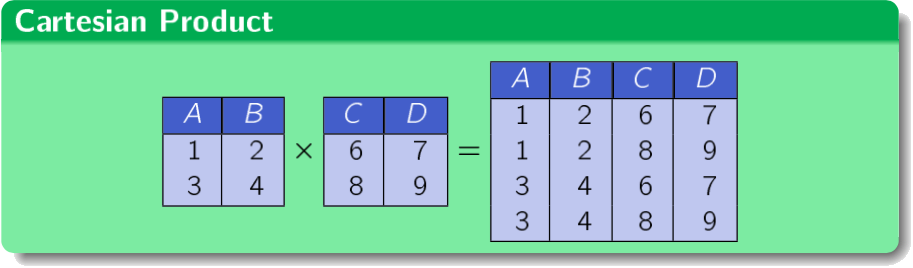
\includegraphics[width= 250pt]{tex/lecture2/cartesianproduct.png}
\end{center}
\subsubsection{Join}





























\/*
\section*{Relational Models \& Algebra}
Schema in a database: structure of the DB = relations + constraints
\\For example, for a Customer(id number, name, street, city), we can say that the primary key constraint is on the id number. It can be used as the primary key, as the id should be unique, whereas multiple customers can share the same name, street or address
\\We can use constraints in different ways. We can constrain the datatypes for a given field, for example an id number should not allow letters.  
\subsection*{Relation Schema}
A relation schema $s$ (a.k.a the schema of a single relation) defines the following:
\begin{itemize}
    \item a (finite) sequence $A_1,...,A_n$ of \textbf{attribute names}
    \begin{itemize}
        \item these names must be distinct
        \item i.e. $A_i \neq A_j$ for $i \neq j$
    \end{itemize}
    \item For each attribute $A_i$, a data type (or \textbf{domain}) $D_i$
    \begin{itemize}
        \item for each A, we let $domain(A_i):= value(D_i)$
    \end{itemize}
    \item We can write this schema as $$s = (A_1 : D_1,...,A_n : D_n)$$
\end{itemize}

\section*{Shit we can do with tables}
\subsection*{Join}
\subsubsection*{Inner}
Returns records that have matching values in both tables
\begin{table}
\begin{center}
 \begin{tabular}{|c c c c|} 
 \hline
 Col1 & Col2 & Col3 & Col4 \\ [0.5ex] 
 \hline\hline
 1 & 6 & 87837 & 787 \\ 
 \hline
 2 & 7 & 78 & 5415 \\
 \hline
 3 & 545 & 778 & 7507 \\
 \hline
 4 & 545 & 18744 & 7560 \\
 \hline
 5 & 88 & 788 & 6344 \\ [1ex] 
 \hline
 
\end{tabular}
\end{center}
\caption{table1}
\end{table}
\begin{table}
\begin{center}
\begin{tabular}{|c c c c|} 
 \hline
 Col1 & Col2 & Col5 & Col6 \\ [0.5ex] 
 \hline\hline
 14 & 62 & 837 & 77 \\ 
 \hline
 22 & 723 & 7854 & 54 \\
 \hline
 312 & 55 & 7748 & 717 \\
 \hline
 454 & 5 & 1384 & 60 \\
 \hline
 534 & 658 & 7348 & 623144 \\ [1ex] 
 \hline
 
\end{tabular}
\end{center}
\caption{table2}
\end{table}
\begin{lstlisting}[language=SQL]
SELECT table1.Col1, table2.Col5, table1.Col3 
FROM Orders 
INNER JOIN table1 ON table1.Col1=table1.Col1;
\end{lstlisting}
\subsubsection*{Left Outer}
\subsubsection*{Right Outer}
\subsubsection*{Full Outer}
*/
\end{document}
